\documentclass[conference]{IEEEtran}
\IEEEoverridecommandlockouts
% The preceding line is only needed to identify funding in the first footnote. If that is unneeded, please comment it out.
\usepackage{cite}
\usepackage{amsmath,amssymb,amsfonts}
\usepackage{algorithmic}
\usepackage{graphicx}
\usepackage{textcomp}
\usepackage{xcolor}
\usepackage{multirow}
\usepackage{rotating}
\usepackage{mdframed}
\usepackage{hyperref}
\usepackage{tikz}
\usepackage{makecell}
\usepackage{tcolorbox}
\usepackage{amsthm}
%\usepackage[english]{babel}
\usepackage{pifont} % checkmarks
%\theoremstyle{definition}
%\newtheorem{definition}{Definition}[section]


\usepackage{listings}
\lstset
{ 
    basicstyle=\footnotesize,
    numbers=left,
    stepnumber=1,
    xleftmargin=5.0ex,
}

%SCJ
\usepackage{subcaption}
\usepackage{array, multirow}
\usepackage{enumitem}


\newcolumntype{U}{>{\columncolor{ucgray}\bfseries\raggedright\arraybackslash}p{0.12\columnwidth}}
\newcolumntype{B}{>{\raggedright\arraybackslash}X}
% --- Use case tables ---------------------------------------------------
\usepackage{tabularx}
\usepackage{colortbl}
\definecolor{ucgray}{gray}{0.92}
\newcolumntype{L}{>{\columncolor{ucgray}\bfseries\raggedright\arraybackslash}p{0.20\columnwidth}}
\newcolumntype{Y}{>{\raggedright\arraybackslash}X}
\newcounter{ucstep}
\newenvironment{ucsteps}{%
  \begin{minipage}[t]{\linewidth}\raggedright%
  \setcounter{ucstep}{0}%
  \def\item{\par\stepcounter{ucstep}\hangindent=1.4em\hangafter=1%
    \noindent\makebox[1.4em][l]{\theucstep.}\ignorespaces}%
}{%
  \strut\end{minipage}%
}
% \usecase{ID}{Name}{Actor}{Description}{Preconditions}{Main flow}{Postconditions}
\newcommand{\usecase}[6]{%
  \begin{table}[htbp]
    \centering
    \caption{#1: #2}
    \label{tab:#1}
    \footnotesize
    \renewcommand{\arraystretch}{1.3}%
    \begin{tabularx}{\columnwidth}{|L|Y|}
      \hline
      Actors         & #3 \\ \hline
      Preconditions  & #4 \\ \hline
      Steps          & #5 \\ \hline
      Postconditions & #6 \\ \hline
    \end{tabularx}
  \end{table}%
}
% ------------------------------------------------------------------------
\newcommand{\rx}{\textcolor{red}{\textbf{X}}}

\def\BibTeX{{\rm B\kern-.05em{\sc i\kern-.025em b}\kern-.08em
    T\kern-.1667em\lower.7ex\hbox{E}\kern-.125emX}}
\begin{document}

%\IEEEpubid{978-1-6654-8356-8/22/\$31.00 ©2022 IEEE}
% @Sune:
% Found this suggestion: https://site.ieee.org/compel2018/ieee-copyright-notice/
% I have added it - you can see if it fulfills the requirements

%\IEEEoverridecommandlockouts
%\IEEEpubid{\makebox[\columnwidth]{978-1-6654-8356-8/22/\$31.00 ©2022 IEEE %\hfill} \hspace{\columnsep}\makebox[\columnwidth]{ }}
                                 %978-1-6654-8356-8/22/$31.00 ©2022 IEEE
% copyright notice added:
%\makeatletter
%\setlength{\footskip}{20pt} 
%\def\ps@IEEEtitlepagestyle{%
%  \def\@oddfoot{\mycopyrightnotice}%
%  \def\@evenfoot{}%
%}
%\def\mycopyrightnotice{%
%  {\footnotesize 978-1-6654-8356-8/22/\$31.00 ©2022 IEEE\hfill}% <--- Change here
%  \gdef\mycopyrightnotice{}% just in case
%}
      
\title{NRGels - The State of Gel Production\\
}

\author{
    \IEEEauthorblockN{
        Christina Gravy\IEEEauthorrefmark{1},
        David Frederik Hulstrøm\IEEEauthorrefmark{1},
        Emil Kjær Fuglsang\IEEEauthorrefmark{1},
        Mads Bundgaard Jeppesen\IEEEauthorrefmark{1},
        Maksymilian Grobicki-Madej\IEEEauthorrefmark{1},
    }
    \IEEEauthorblockA{
        University of Southern Denmark, SDU Software Engineering, Odense, Denmark \\
        Email: \IEEEauthorrefmark{1} \textnormal{\{chgre23@student.sdu.dk,dahul23@student.sdu.dk,emfug23@student.sdu.dk,majep23@student.sdu.dk,mgrob26@student.sdu.dk\}}@mmmi.sdu.dk
    }
}


%%%%

%\author{\IEEEauthorblockN{1\textsuperscript{st} Blinded for review}
%\IEEEauthorblockA{\textit{Blinded for review} \\
%\textit{Blinded for review}\\
%Blinded for review \\
%Blinded for review}
%\and
%\IEEEauthorblockN{2\textsuperscript{nd} Blinded for review}
%\IEEEauthorblockA{\textit{Blinded for review} \\
%\textit{Blinded for review}\\
%Blinded for review \\
%Blinded for review}
%\and
%\IEEEauthorblockN{3\textsuperscript{nd} Blinded for review}
%\IEEEauthorblockA{\textit{Blinded for review} \\
%\textit{Blinded for review}\\
%Blinded for review \\
%Blinded for review}
%}

%%%%
%\IEEEauthorblockN{2\textsuperscript{nd} Given Name Surname}
%\IEEEauthorblockA{\textit{dept. name of organization (of Aff.)} \\
%\textit{name of organization (of Aff.)}\\
%City, Country \\
%email address or ORCID}

\maketitle
\IEEEpubidadjcol
\begin{abstract}
%%%%%%%%%%%%%%%%%% Max 970 signs without space %%%%%%%%%%%%%%%%%%
% Intro

% Gab
    
% Aim 

% Method

% Results 

\end{abstract}

\begin{IEEEkeywords}
Keyword1, Keyword2, Keyword3, Keyword4, Keyword5
\end{IEEEkeywords}

\section{Introduction and Motivation}
%Introduction and motivate the problem

The structure of the paper is as follows. 
Section \ref{sec:problem} outlines the research question and the research approach. 
%to analyze the research question and evaluate our results.
Section \ref{sec:related_work} describes similar work in the field and how our contribution fits the field.
Section \ref{sec:use_case} presents a production reconfiguration use case.
The use case serves as input to specify a reconfigurability QA requirement in Section \ref{sec:qas}.
Section \ref{sec:middleware_architecture} introduces the proposed reconfigurable middleware software architecture design.
Section \ref{sec:evaluation} evaluates the proposed middleware on realistic equipment in the I4.0 lab and analyzes the results against the stated QA requirement.   

% Placeholder text
Lorem ipsum dolor sit amet, consectetur adipiscing elit, sed do eiusmod tempor incididunt ut labore et dolore magna aliqua. Ut enim ad minim veniam, quis nostrud exercitation ullamco laboris nisi ut aliquip ex ea commodo consequat. Duis aute irure dolor in reprehenderit in voluptate velit esse cillum dolore eu fugiat nulla pariatur.

\section{Problem and Approach}

\label{sec:problem}
\emph{Problem.}
\begin{table}[htbp]
  \centering
  \caption{Functional Requirements}
  \label{tab:functional_requirements}
  \footnotesize
  \renewcommand{\arraystretch}{1.3}
  \begin{tabularx}{\columnwidth}{|U|B|}
    \hline
    \rowcolor{ucgray}\textbf{ID} & \textbf{Functional Requirement} \\ \hline
    FR-1 & Production software must be able to exchange and coordinate information to execute a production and change production. \\ \hline
    FR-2 & Routine machine data is sent to machine suppliers every 12 hours. \\ \hline
    FR-3 & A maintenance request is sent to a machine supplier if a machine breaks. \\ \hline
    FR-4 & The coordination system can accommodate machines slowing down or halting. \\ \hline
    FR-5 & The production system can produce 3 different flavoured gels simultaneously. \\ \hline
    FR-6 & A resource order is sent when the warehouse stock levels are low. \\ \hline
    FR-7 & Product manager can schedule a production run. \\ \hline
  \end{tabularx}
\end{table}

\begin{table}[htbp]
  \centering
  \caption{Non-Functional Requirements}
  \label{tab:non_functional_requirements}
  \footnotesize
  \renewcommand{\arraystretch}{1.3}
  \begin{tabularx}{\columnwidth}{|U|B|}
    \hline
    \rowcolor{ucgray}\textbf{ID} & \textbf{Non-Functional Requirement} \\ \hline
    NFR-1 & Production software must run 24/7. \\ \hline
    NFR-2 & Production software must be continuously deployable. \\ \hline
    NFR-3 & The production software should be reconfigurable. \\ \hline
    NFR-4 & Unsealed gel wrappers are not exposed to the air for longer than 10 minutes. \\ \hline
    NFR-5 & Production software’s SLA at 99.9\% \\ \hline
  \end{tabularx}
\end{table}

\emph{Research questions:}
\begin{enumerate}
    \item  
    \item 
\end{enumerate}

\emph{Approach.}
The following steps are taken to answer this paper's research questions: 
\begin{enumerate}
    \item 
\end{enumerate}

% Placeholder text
Sed ut perspiciatis unde omnis iste natus error sit voluptatem accusantium doloremque laudantium, totam rem aperiam, eaque ipsa quae ab illo inventore veritatis et quasi architecto beatae vitae dicta sunt explicabo. Nemo enim ipsam voluptatem quia voluptas sit aspernatur aut odit aut fugit, sed quia consequuntur magni dolores eos qui ratione voluptatem sequi nesciunt.

\section{Related work}
\label{sec:related_work}
This Section addresses existing contributions by examining xxx in the I4.0 domain. 
In total, x papers are investigated. 

In \cite{Wan2019Reconfigurable}, experiences are elaborated on a three-layer architecture of a reconfigurable smart factory for drug packing in healthcare I4.0. 

The paper \cite{Yazen2010Ontology} proposes an ontology agent-based architecture for inferring  new configurations to adapt to changes in manufacturing requirements and/or environment.

In \cite{Leitao2016Specification,Angione2017Integration} an architecture for a reconfigurable production system is specified.
Two objectives for reconfiguration and how they can be reached are described.

Several papers \cite{Koren1999Reconfigurable,Koren2010Design,Bortolini2018Reconfigurable} describe reconfigurable manufacturing systems that are cost-effective and responsive to market changes.

All contributions provide valuable knowledge about reconfiguration but lack a study of the software architecture perspective that specifies a quantifiable reconfigurability architectural requirement, a software architecture that adopts the architectural requirements, and evaluates the architectural requirement. 

% Placeholder text
At vero eos et accusamus et iusto odio dignissimos ducimus qui blanditiis praesentium voluptatum deleniti atque corrupti quos dolores et quas molestias excepturi sint occaecati cupiditate non provident. Similique sunt in culpa qui officia deserunt mollitia animi, id est laborum et dolorum fuga.

\section{Use Case}
\label{sec:use_case}
This Section introduces the use cases.
Tables~\ref{tab:UC-1}--\ref{tab:UC-7} present the use cases.

\usecase{UC-1}{Schedule Production Run}
  {Production Manager, Scheduling System}
  {A verified production order exists.}
  {%
    \begin{ucsteps}
      \item Production Manager logs into the Scheduling System.
      \item Production Manager selects the ”Schedule Production Run” option.
      \item The Scheduling System fetches available time slots and resources.
      \item Production Manager selects appropriate time slot and resources.
      \item The Scheduling System confirms the schedule and notifies related components.
    \end{ucsteps}%
  }
  {The schedule is updated and now includes the new production run. The planned use of resources is updated.}

\usecase{UC-2}{Warn if scheduled production run is low on resources}
  {Production Manager, Scheduling System}
  {A new production is being planned and not enough resources are available.}
  {%
    \begin{ucsteps}
      \item Production Manager logs into the Scheduling System.
      \item Production Manager selects the ”Schedule Production Run” option.
      \item Production Manager inputs wanted batch production, larger than currently available resources. \rx %the steps should mirror uc1?
      \item Production Manager selects appropriate time slot and resources.
      \item The Scheduling System warns the Production Manager, and refuses to schedule the production.
    \end{ucsteps}%
  }
  {The production run is not scheduled, and the Production Manager is notified.}

\usecase{UC-3}{Production Coordination System sends Resource Order to Warehouse}
  {Production Coordination System, Warehouse}
  {Stock levels of a material is under threshold on the Production Line. No PENDING Resource order.}
  {%
    \begin{ucsteps}
      \item A machine sends a low-stock message.
      \item Monitoring System captures low-stock message.
      \item Monitoring system checks if the material is PENDING from Warehouse.
      \item The system requests new materials from warehouse. \rx %who is 'the system' - PCS?
      \item Upon confirmation, the system marks the material PENDING. 
    \end{ucsteps}%
  }
  {A resource order is sent to and confirmed by the warehouse. Production Manager is notified.}

\usecase{UC-4}{Overload causes slow-down for tapping}
  {Gel Tapper, Gel Sealer, Production Coordination System (PCS)}
  {Flavoured gel is mixed and ready to be tapped into wrappers. The sealer is in an overload state.}
  {%
    \begin{ucsteps}
      \item Sealer sends OVERLOAD message.
      \item Production Coordination System captures OVERLOAD message.
      \item PCS sends a HALT message to the tapping station.
      \item Tapping station halts to avoid generating unsealed, exposed gels.
      \item Sealer sends READY message.
      \item PCS captures READY message and sends START message to tapping station.
      \item Tapping station resumes action.
    \end{ucsteps}%
  }
  {Normal production is resumed.}

\usecase{UC-5}{Handle machine failure}
  {Monitoring System, Machine Supplier}
  {A machine is malfunctioning.}
  {%
    \begin{ucsteps}
      \item A machine stops sending sensor data or is unresponsive. \rx % sensor data - heartbeats?
      \item The error is detected by the Monitoring System.
      \item A maintenance or repair request is sent to the machine supplier.
      \item Confirmation message is sent by the machine supplier.
      \item A trigger message for swapping to a spare machine in the production line.
    \end{ucsteps}%
  }
  {Production continues as normal, with the malfunctioning machine being swapped out.}

\usecase{UC-6}{Logging machine metrics}
  {Monitoring System, Machines}
  {The machines are running.}
  {%
    \begin{ucsteps}
      \item Timestamped metrics (Temperature, speed, etc.) are sent by the machines.
      \item The Monitoring System captures and stores the events
    \end{ucsteps}%
  }
  {Timestamped metrics are persisted.}

\usecase{UC-7}{Sending routine data to the machine supplier}
  {Machine supplier, Monitoring System}
  {Machine data has been collected for 24 hours.}
  {%
    \begin{ucsteps}
      \item Routine data is retrieved.
      \item Routine data is aggregated.
      \item The processed data is sent to the machine suppliers.
    \end{ucsteps}%
  }
  {A notification is sent to the machine supplier.}

% Placeholder text
Nam libero tempore, cum soluta nobis est eligendi optio cumque nihil impedit quo minus id quod maxime placeat facere possimus, omnis voluptas assumenda est, omnis dolor repellendus. Temporibus autem quibusdam et aut officiis debitis aut rerum necessitatibus saepe eveniet ut et voluptates repudiandae sint et molestiae non recusandae.

\section{Quality Attribute Scenario}
\label{sec:qas}
This Section introduces the specified x QASes.
The QASes are developed based on the use case.
Table~\ref{tab:QAS} presents the QAS and Table~\ref{tab:constraints} lists the constraints.

\begin{table}[htbp]
  \centering
  \caption{Quality Attribute Scenarios}
  \label{tab:QAS}
  \footnotesize
  \renewcommand{\arraystretch}{1.3}
  % Columns: ID (narrow, gray) | QA | Scenario (takes remaining width) | Associated Use Case
  \setlength{\tabcolsep}{4pt}% tighter cell padding leaves more room for Scenario
  \begin{tabularx}{\columnwidth}{|>{\columncolor{ucgray}\bfseries\raggedright\arraybackslash}p{0.10\columnwidth}|>{\raggedright\arraybackslash\hspace{0pt}}p{0.20\columnwidth}|Y|>{\raggedright\arraybackslash\hspace{0pt}}p{0.12\columnwidth}|}
    \hline
    \rowcolor{ucgray}\textbf{ID} & \textbf{QA} & \textbf{Scenario} & \textbf{Assoc.\ UC or CON} \\ \hline
    QA-1 & Availability & When the stock level falls below the threshold, it is detected within 10s and a message is sent to the warehouse within 100 ms. & UC-3 \\ \hline
    QA-2 & Availability & Upon a machine failing, it should be detected within 100 ms and a repair request sent within 50 ms of detecting the failure. & UC-5 \\ \hline
    QA-3 & Availability & Production software’s SLA at 99.9\% availability. & All \\ \hline
    QA-4 & Availability & Upon a software system failure a replacement service is running within 1 minute. & All \\ \hline
    QA-5 & Scalability & The system will initially support metrics ingestion from 50 machines and should be capable of handling metrics from up to 500 machines without increasing average latency by more than 25\% and the P95 by 200\%. & UC-6 \\ \hline
    QA-6 & Performance & The condition of the gel sealer is monitored and upon getting overloaded, a message is processed (Production Coordination System receives a message and generates a message which is received by the machine) within 1s. & CON-4 \\ \hline
    QA-7 & Performance & Scheduled production runs are persisted within 100ms. & UC-1 \\ \hline
    QA-8 & Performance & The stock levels are fetched within 1s. & UC-2 \\ \hline
    QA-9 & Security & The Scheduling System is only available for registered users with a username and password. & UC-1  UC-2 \\ \hline
    QA-10 & Interoperability & Machines and services can communicate regardless of their protocol without changes to the existing software. & All \\ \hline
    QA-11 & Modifiability & New machines can be integrated into the existing system, without changing the current software. & All \\ \hline
    QA-12 & Safety & Unsealed gels are never exposed for more than 10 minutes. & UC-4 \\ \hline
  \end{tabularx}
\end{table}

\begin{table}[htbp]
  \centering
  \caption{Constraints}
  \label{tab:constraints}
  \footnotesize
  \renewcommand{\arraystretch}{1.3}
  \begin{tabularx}{\columnwidth}{|U|B|}
    \hline
    \rowcolor{ucgray}\textbf{ID} & \textbf{Constraint} \\ \hline
    CON-1 & Production Software must run 24/7. \\ \hline
    CON-2 & Production Software must be continuously deployable. \\ \hline
    CON-3 & Production software must be able to exchange and coordinate information to execute a production and change production. \\ \hline
    CON-4 & Users interact with the production software through a web browser. \\ \hline
  \end{tabularx}
\end{table}

% Description of the overall architecture designs
% Argue for tactics used to archieve the QASes
% Discuss the trade-offs
\section{Design and Analysis Modelling}
\label{sec:design_and_analysis_modelling}
Design and analysis modelling.


\begin{figure}[htbp]
  \centering
  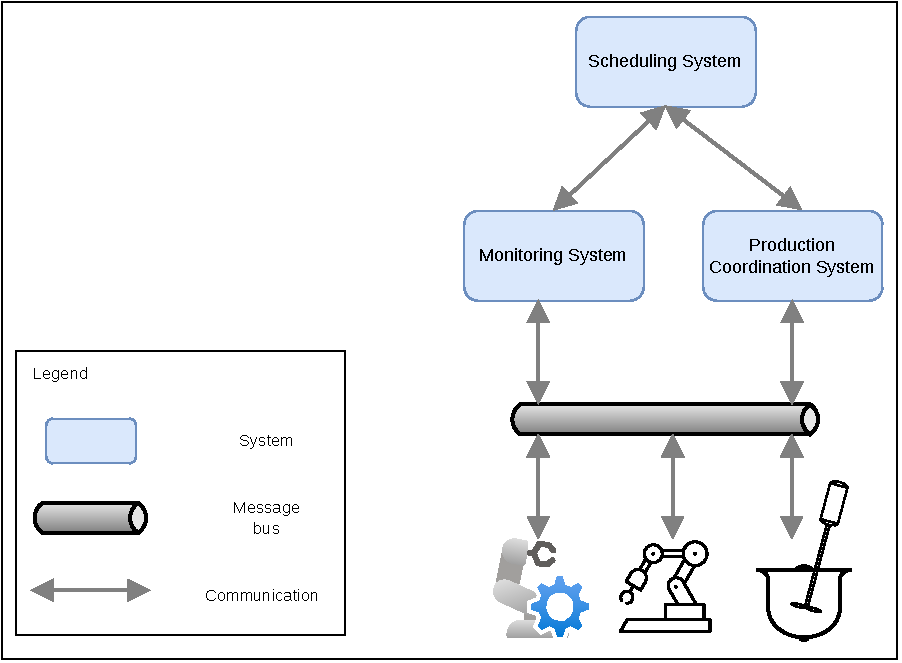
\includegraphics[width=\columnwidth]{img/architecture_overview.pdf}
  \caption{Overview of the architecture}
  \label{fig:architecture-diagram}
\end{figure}

% Placeholder text
Sed ut perspiciatis unde omnis iste natus error sit voluptatem accusantium doloremque laudantium, totam rem aperiam, eaque ipsa quae ab illo inventore veritatis et quasi architecto beatae vitae dicta sunt explicabo. Nemo enim ipsam voluptatem quia voluptas sit aspernatur aut odit aut fugit, sed quia consequuntur magni dolores eos qui ratione voluptatem sequi nesciunt.

\section{Formal verification and validation}
\label{sec:formal_v_and_v}
Formal verification and validation of system(s).

% Placeholder text
At vero eos et accusamus et iusto odio dignissimos ducimus qui blanditiis praesentium voluptatum deleniti atque corrupti quos dolores et quas molestias excepturi sint occaecati cupiditate non provident. Similique sunt in culpa qui officia deserunt mollitia animi, id est laborum et dolorum fuga.

\section{Evaluation}
\label{sec:evaluation}

% Empirical evaluation
This Section describes the evaluation of the proposed design.
Section \ref{sec:design} introduces the design of the experiment to evaluate the system. 
Section \ref{sec:measurements} identifies the measurements in the system for the experiment.
Section \ref{sec:pilot_test} describes the pilot test used to compute the number of replication in the actual evaluation. 
Section \ref{sec:analysis} presents the analysis of the results from the experiment. 

% Placeholder text
Nam libero tempore, cum soluta nobis est eligendi optio cumque nihil impedit quo minus id quod maxime placeat facere possimus, omnis voluptas assumenda est, omnis dolor repellendus. Temporibus autem quibusdam et aut officiis debitis aut rerum necessitatibus saepe eveniet ut et voluptates repudiandae sint et molestiae non recusandae.

\subsection{Experiment design}
\label{sec:design}

% Placeholder text
Lorem ipsum dolor sit amet, consectetur adipiscing elit, sed do eiusmod tempor incididunt ut labore et dolore magna aliqua. Ut enim ad minim veniam, quis nostrud exercitation ullamco laboris nisi ut aliquip ex ea commodo consequat. Duis aute irure dolor in reprehenderit in voluptate velit esse cillum dolore eu fugiat nulla pariatur.

\subsection{Measurements}
\label{sec:measurements}

% Placeholder text
Sed ut perspiciatis unde omnis iste natus error sit voluptatem accusantium doloremque laudantium, totam rem aperiam, eaque ipsa quae ab illo inventore veritatis et quasi architecto beatae vitae dicta sunt explicabo. Nemo enim ipsam voluptatem quia voluptas sit aspernatur aut odit aut fugit, sed quia consequuntur magni dolores eos qui ratione voluptatem sequi nesciunt.

\subsection{Pilot test}
\label{sec:pilot_test}

% Placeholder text
At vero eos et accusamus et iusto odio dignissimos ducimus qui blanditiis praesentium voluptatum deleniti atque corrupti quos dolores et quas molestias excepturi sint occaecati cupiditate non provident. Similique sunt in culpa qui officia deserunt mollitia animi, id est laborum et dolorum fuga.

\subsection{Analysis}
\label{sec:analysis}

% Placeholder text
Nam libero tempore, cum soluta nobis est eligendi optio cumque nihil impedit quo minus id quod maxime placeat facere possimus, omnis voluptas assumenda est, omnis dolor repellendus. Temporibus autem quibusdam et aut officiis debitis aut rerum necessitatibus saepe eveniet ut et voluptates repudiandae sint et molestiae non recusandae.

\section{Conclusion}
\label{sec:conclusion}
Conclusion of the report, discussion and relevant future work.

% Placeholder text
Lorem ipsum dolor sit amet, consectetur adipiscing elit, sed do eiusmod tempor incididunt ut labore et dolore magna aliqua. Ut enim ad minim veniam, quis nostrud exercitation ullamco laboris nisi ut aliquip ex ea commodo consequat. Duis aute irure dolor in reprehenderit in voluptate velit esse cillum dolore eu fugiat nulla pariatur.

\subsection{Discussion}
\label{sec:Discussion}

% Placeholder text
Sed ut perspiciatis unde omnis iste natus error sit voluptatem accusantium doloremque laudantium, totam rem aperiam, eaque ipsa quae ab illo inventore veritatis et quasi architecto beatae vitae dicta sunt explicabo. Nemo enim ipsam voluptatem quia voluptas sit aspernatur aut odit aut fugit, sed quia consequuntur magni dolores eos qui ratione voluptatem sequi nesciunt.

\subsection{Future work}
\label{sec:future_work}

% Placeholder text
At vero eos et accusamus et iusto odio dignissimos ducimus qui blanditiis praesentium voluptatum deleniti atque corrupti quos dolores et quas molestias excepturi sint occaecati cupiditate non provident. Similique sunt in culpa qui officia deserunt mollitia animi, id est laborum et dolorum fuga.

\bibliographystyle{IEEEtran}
\bibliography{references}
\vspace{12pt}

\newpage
\section*{Contributions}
\begin{tabular}{l|p{0.6\linewidth}}
Name & Contribution\\
\end{tabular}
\end{document}
